% !TeX root = ../main.tex
\chapter{绪论}

\section{研究的背景和意义}

随着互联网的发展,互联网数据中心(Internet Data Center,IDC)在世界各地兴起。21 世纪第一个十年,数据中心主要处理 Web 网站、搜索引擎等容易并行的任务。因此,互联网数据中心多使用大量低成本的标准服务器搭建。

近十年来,大数据处理与机器学习的兴起改变了数据中心的负载特性。一方面,大数据处理、机器学习等负载对算力要求很高。然而,由于 Dennard 缩放定律的终结,近十年来,通用处理器的频率提升和多核核数增加都受到功耗墙的限制。因此,通用处理器性能提升 ``免费的午餐'' 已经结束,体系结构的创新迎来了春天,GPU、FPGA、TPU 等定制化硬件在数据中心内大量部署。另一方面,大数据处理、机器学习等负载需要多个节点紧密协同处理,对节点间的通信带宽和延迟要求较高。因此,近十年来,数据中心网络从 1 Gbps 发展到 40 Gbps,并有向 100 Gbps 演进的趋势。定制化硬件之间的专用互连也成为趋势。因此,如英伟达 CEO 黄仁勋所说,未来的数据中心会像超级计算机一样。

与此同时,数据中心的运营模式也在经历一场云化的变革。数据中心的算力逐渐集中到少数几家云厂商,每家拥有数以百万计的服务器。





\begin{figure}[htbp]
	\centering
	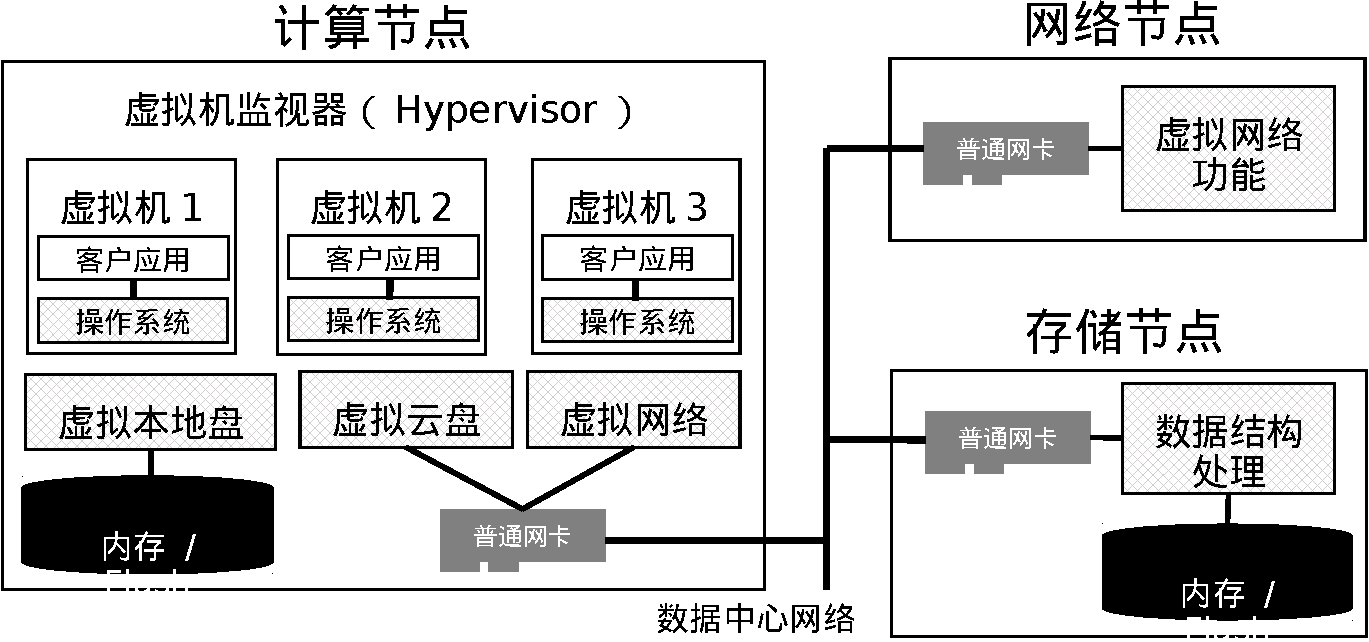
\includegraphics[width=0.8\textwidth]{figures/virt_arch.pdf}
	\caption{虚拟化的数据中心架构。}
	\label{background:fig:virt-architecture}
\end{figure}

\section{国内外研究现状}




第二章提炼 2 页

\section{本文的研究内容和贡献}



\begin{figure}[htbp]
	\centering
	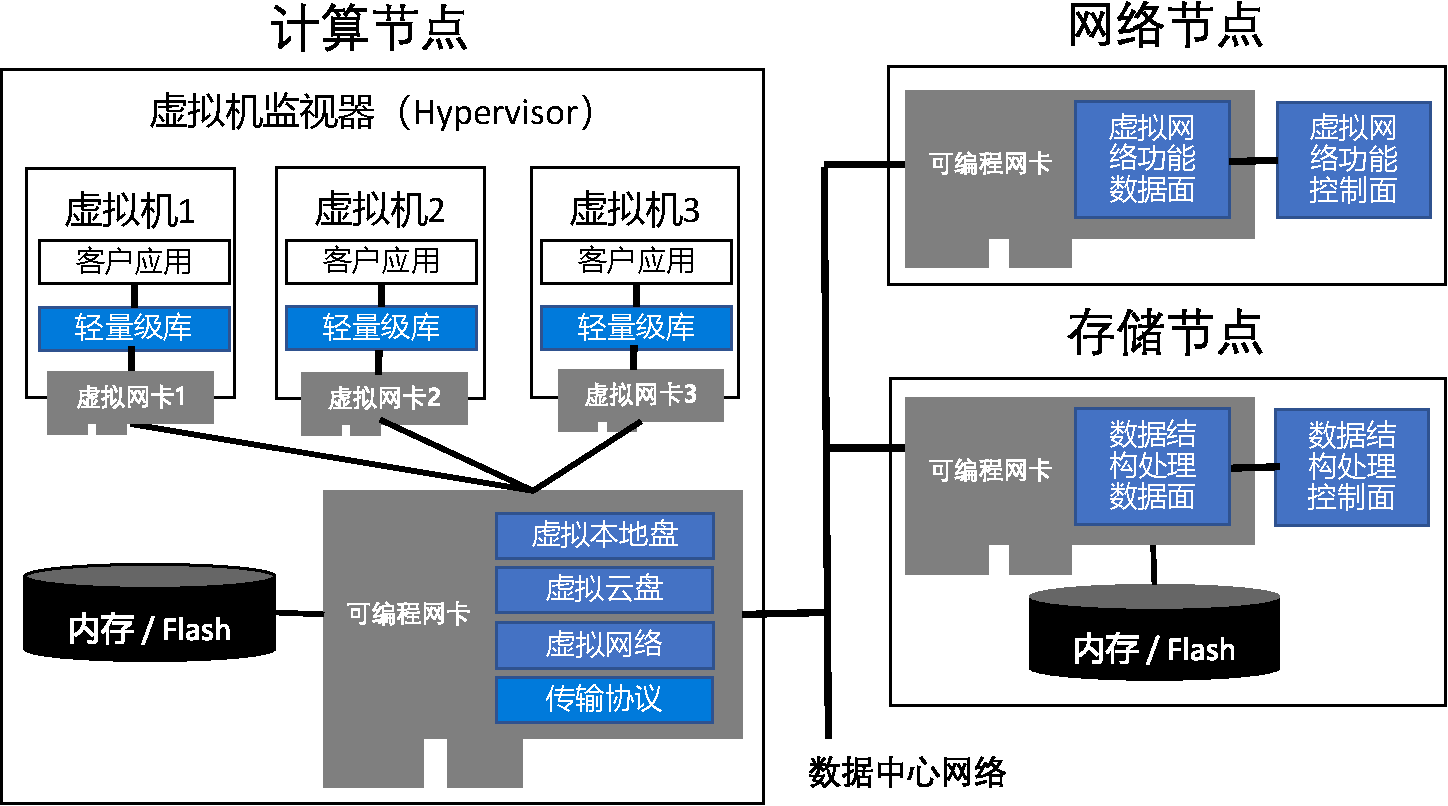
\includegraphics[width=0.8\textwidth]{figures/accel_arch.pdf}
	\caption{基于可编程网卡的数据中心系统总体架构。}
	\label{arch:fig:accel-arch}
\end{figure}

摘要的扩充,第三章提炼 2 页

\section{论文结构安排}

本论⽂的内容结构安排如下:
第 1 章为绪论。
第 2 章介绍了数据中心的背景知识和硬件的发展趋势,分析了可编程网卡的四种架构,并调研了可编程网卡在数据中心的应用。
第 3 章提出了基于可编程网卡的高性能数据中心系统架构。
第 4 章提出用可编程网卡加速云计算中的虚拟网络功能。为了简化FPGA编程,提出了首个适用于高速网络数据包处理、基于高级语言的模块化FPGA编程框架ClickNP。
第 5 章提出用可编程网卡加速远程数据结构访问,并设计实现了一个高性能内存键值存储系统 KV-Direct。
第 6 章提出用可编程网卡和用户态运行库相结合的方法为应用程序提供操作系统原语,并设计实现了一个用户态套接字系统 SocksDirect。
第 7 章总结全⽂并展望未来研究方向。